
\section{Uživatelské rozhraní}
Tato sekce se zabývá architekturou a implementací uživatelského rozhraní formou webové stránky. Implementace je rozdělena do dvou balíčků:
\begin{itemize}
    \item Framework-ui - obsahuje komplexní řešení pro validace formulářů včetně integrace s Redux (napojení na state, definice akcí a reducerů), implementuje znovu použitelné React komponenty, včetně komponenty řešící přímé napojení formulářového pole na state a obsluhu jeho validací (FieldConnector). Dále jazykovou lokalizaci pro systémové hlášky a nádstavbu nad základní rozhraní pro odesílání HTTP požadavků, která řeší zobrazení chybových hlášek a definuje flexibilnější rozhraní.
    \item Frontend - implementace samotné aplikace
\end{itemize}

\subsection{Frontend}
Uživatelské rozhraní je realizováno jako SPA - průchod celou aplikací je plynulý a nikdy nedochází k přenačítání celé stránky, ale pouze k překreslení potřebných částí. Toto řešení zlepšuje uživatelský zážitek, protože stránka zůstává pořád plně aktivní a při čekání na vyřízení požadavku uživatel může pokračovat v interakci. Také je zde implementován standard PWA - v podporovaných systémech jako je např. android lze aplikaci tzv. \uv{Přidat na plochu}, potom při otevření vypadá jako nativní aplikace (nemá zobrazený url bar). Statické soubory jsou v cache, díky čemuž je minimalizován datový přenost a stav aplikace je perzistentně ukládán, takže při zavření aplikace a následném otevření je stav plně obnoven a uživatel pokračuje přesně tam, kde skončil naposledy a to i v případě bez přístupu k internetu - aplikace je kompletně načtena, ale následná interakce je již závislá na komunikaci se serverem.

\subsubsection{State management}
React je postavený na předávání dat mezi jednotlivými komponenty, které tvoří stromovou strukturu, data lze však předávat primárně z vrchu dolů a proto je poměrně složité ze spodní komponenty předat změnu do vrchní. Navíc dnešní aplikace pracují s obrovským množstvím dat, ke kterým potřebují přistupovat různé části aplikace a ideálně transparentní cestou data modifikovat a o této modifikaci se musí dozvědět všechny komponenty pracující s danými daty, aby dostali jejich aktuální verzi. Dnes již React obsahuje obecné řešení pro předávání dat, ale já jsem se rozhodl pro využití komplexního řešení s centrálním úložištěm stavu aplikace v podobě knihovny Redux, které nabízí více funkcí a je odzkoušené časem. Redux je založený na \uv{Observer pattern}. Tento návrhový vzor definuje dvě entity - předplatitel (pozorovatel) a vydavatel (pozorovaný). V praxi se jednotlivé komponenty přihlásí k odběru určitých dat (\uv{předplatí si je}) a v případě, že někdo chce data modifikovat, tak se stane vydavatelem a řekne, co modifikuje a jak vypadají nová data. Redux zajistí, že všichni předplatitelé dat, kterých se modifikace týká, dostanou jejich nejnovější verzi. V Reduxu se používá následující terminologie:
\begin{itemize}
    \item store - centrální úložiště dat (tvz. \uv{jediný zdroj pravdy})
    \item akce - popis k jaké změně dojde
    \item dispatch akce - odeslání určité akce k vykonání
    \item reducer - reaguje na odeslanou akci, obsahuje logiky pro modifikaci dat
\end{itemize}
\begin{figure}[htbp]
    \centering
    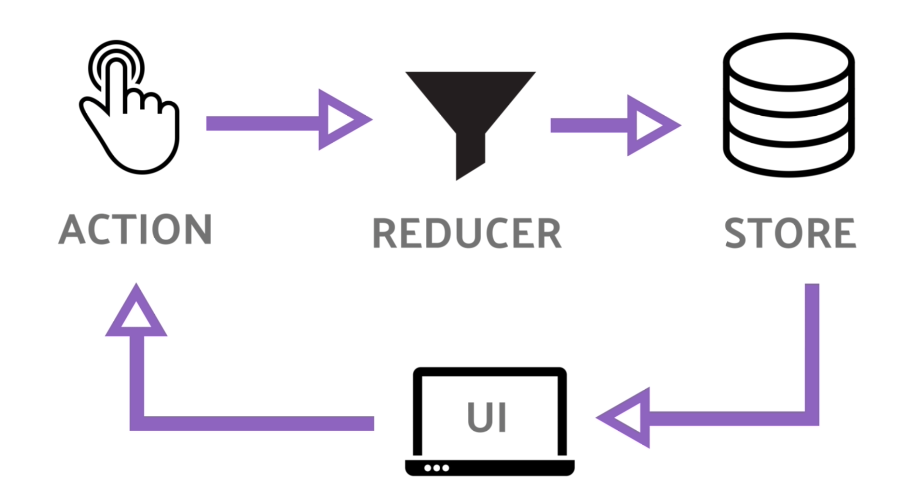
\includegraphics[width=0.5\textwidth]{img/redux.png}
    \caption{Redux tok dat \cite{img-redux-flow}}
\end{figure}

\subsubsection{Vzhled}
V kombinaci s Reactem jsem použil knihovnu Material-ui, která obsahuje velké množství nastylovaných komponent a komplexní řešení pro stylování React komponent. Tuto knihovnu používám již od prvopočátku jejího vzniku a velmi jsem si ji oblíbil kvůli detailní dokumentaci. Obsahuje vestavěné řešení pro \textbf{CSS-in-JS}, které mi jako programátorovi velmi vyhovuje, protože překlenuje spoustu limitací přímého použití CSS. Umožňuje definovat vzhled ve stejném souboru i jazyce jako samotnou React komponentu, díky tomu nemusí programátor přepínat kontext mezi různými jazyky a může se plně soustředit na vývoj uživatelského rozhraní.

\subsection{Souborová struktura}
\dirtree{%
    .1 packages.
    .2 framework-ui.
    .3 src.
    .4 api\DTcomment{implementace rozhraní pro odesílání požadavků}.
    .4 Components\DTcomment{React komponenty}.
    .4 localization\DTcomment{řešení pro lokalizaci systémových hlášek}.
    .4 privileges\DTcomment{pomocné funkce pro oprávnění a jejich dědičnost}.
    .4 redux\DTcomment{implementace akci a reducerů, primárně pro správu formulářových dat}.
    .4 validations\DTcomment{implementace validací}.
    .2 frontend.
    .3 public.
    .3 src.
    .4 Pages\DTcomment{jednotlivé stránky rozhraní}.
    .4 api\DTcomment{definice RESTful volání}.
    .4 components\DTcomment{sdílené komponenty napříč stránkami}.
    .4 containers\DTcomment{React kontejnery obalující celou aplikaci}.
    .4 firebase\DTcomment{služba pro registraci a obsluhu notifikací}.
    .4 store\DTcomment{inicializace Redux, definice akcí a reducerů}.
    .4 webSocket\DTcomment{služba pro inicializaci Socket.IO}.
}

\subsection{Validace}
Obecný princip fungování validací je popsán v sekci \hyperref[BE:Validace]{Backend}. Na Frontendu se validace používají pro upozornění uživatele na případně chybně zadanou hodnotu. Samotná formulářová data jsou spravována knihovnou redux, stejně jako celý state aplikace. Jejich struktura je shodná s deskriptory formuláře - deepPath se využívá pro získání příslušné hodnoty.

Pro vykreslení formulářového pole jsem připravil komponentu \textit{FielConnector}, které se předá typ pole (text, email, select atd.) a deepPath, podle které si nalezne příslušný deskriptor, ze kterého získá potřebné atributy a validace, které se provolávají v následujících případech:
\begin{itemize}
    \item uživatel poprvé zadává hodnotu a vyklikne (událost \uv{onBlur});
    \item uživatel edituje již zadanou hodnotu, potom se validace spouští po každé změně (událost \uv{onChange}).
\end{itemize}

\subsection{Rozhraní}
Aplikace nabízí jednoduché uživatelské rozhraní s jedním menu pro navigaci mezi jednotlivými stránkami a tlačítko pro přihlášení, které otevře přihlašovací dialog.

Nepřihlášenému uživateli je k dispozici stránka pro registraci obsahující formulář. Po registraci je automaticky přihlášen a má k dispozici stránku pro správu zařízení a stránku pro ovládání a sledování jednotlivých věcí. Správa zařízení je rozdělena na dvě sekce, první obsahuje tabulku s detekovanými zařízeními, které lze přidat na dvě kliknutí. Druhá část obsahuje tabulku se zařízeními, ke kterým má uživatel oprávnění pro čtení a v případě oprávnění pro zápis, může editovat jejich informace, měnit oprávnění pro jednotlivé uživatele, odeslat příkaz pro restart nebo zařízení odstranit.

\begin{figure}[htbp]
    \centering
    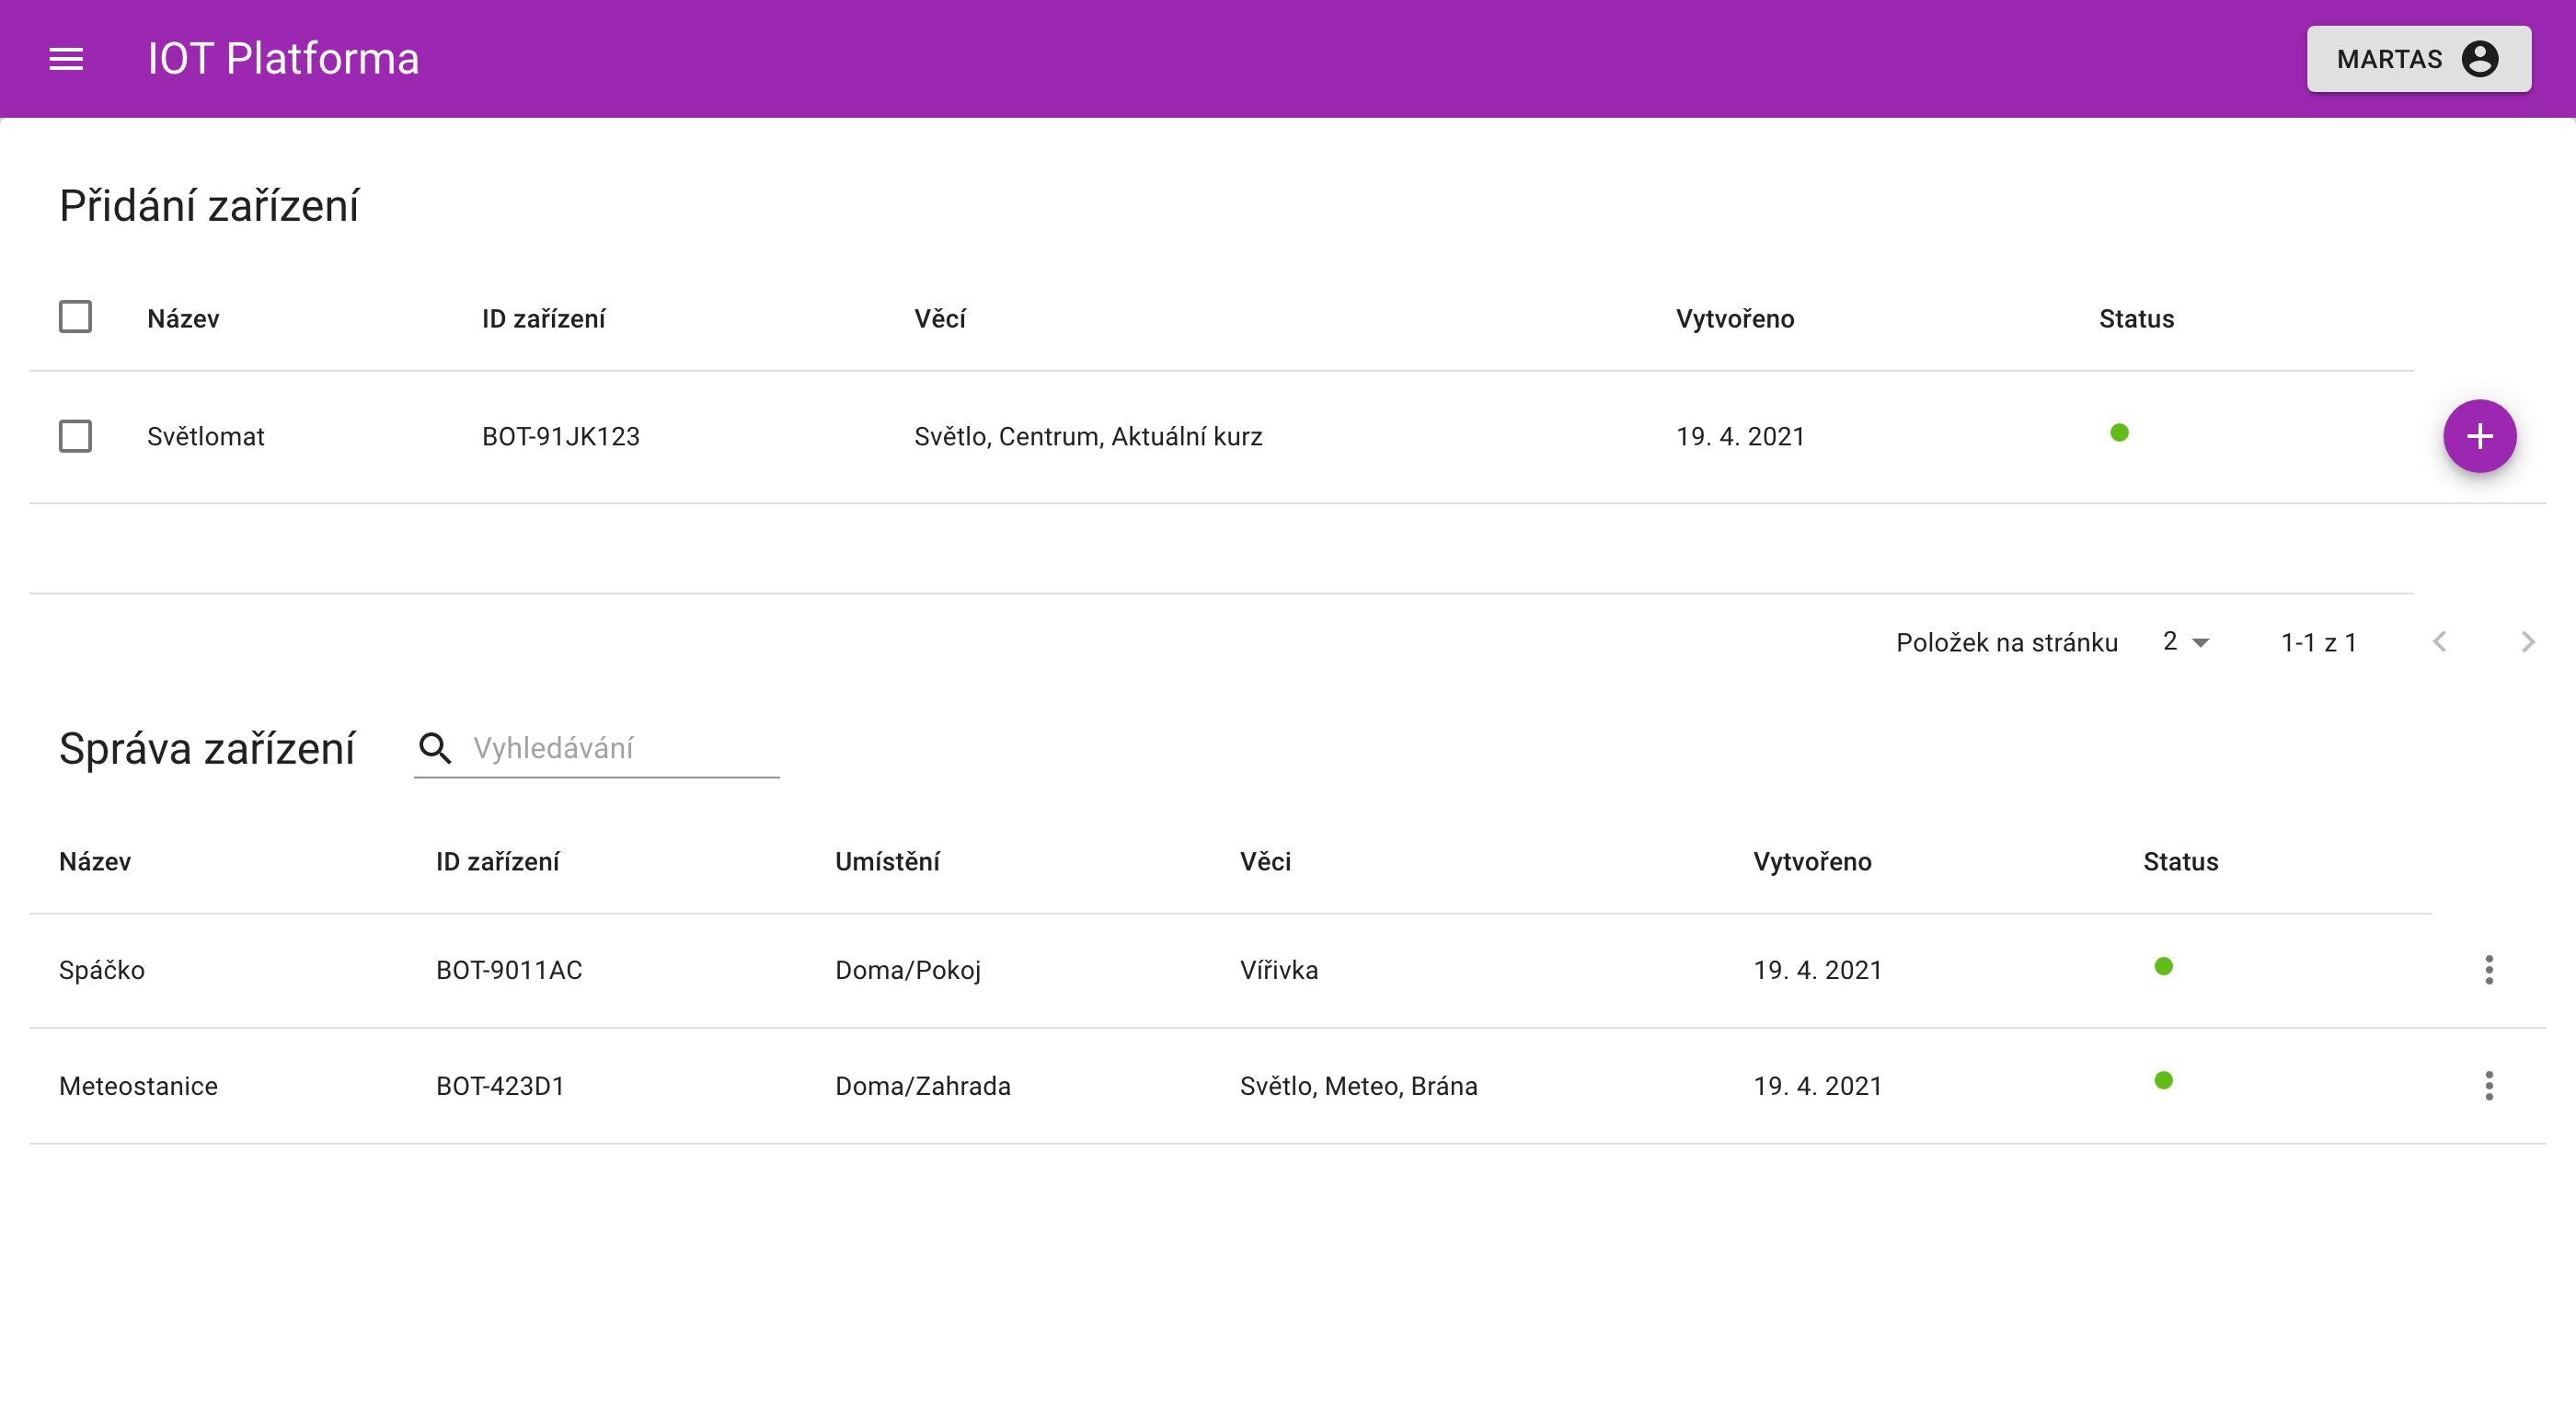
\includegraphics[width=\textwidth]{img/screens/deviceManagement2.png}
    \caption{Ukázka rozhraní - správa zařízení}
\end{figure}

Stránka pro ovládání zobrazuje widgety pro jednotlivé místnosti seskupené podle budov. Pokud místnost obsahuje nějakou věc typu senzor, tak aktuální hodnota je zobrazena na tomto widgetu. Po rozkliknutí místnosti jsou rozbrazeny všechny věci, která daná místnost obsahuje. S některými věcmi lze přímo interagovat (přepínač a aktivátor) a u senzoru je zobrazena aktuální hodnota. Pokud se dané zařízení nenachází v připraveném stavu, tak je uživatel upozorněn barevným kolečkem. Po kliknutí na název věci je zobrazeno dialogové okno, které se částečně liší v závislosti na typu věci:
\begin{itemize}
    \item \textbf{Generic} zobrazí aktuální hodnoty vlastností a je umožněna případná interakce s nimi.
    \item \textbf{Sensor} zobrazí stejný obsah jako pro \textit{generic} a navíc na začátku vykreslený graf vizualizující průběh hodnoty v čase za posledních 24 hodin.
    \item \textbf{Switch} zobrazí stejný obsah jako pro \textit{generic} a navíc časovou osu vizualizující aktivitu vlastnosti.
\end{itemize}

\begin{figure}
    \centering
    \begin{subfigure}{.5\textwidth}
        \centering
        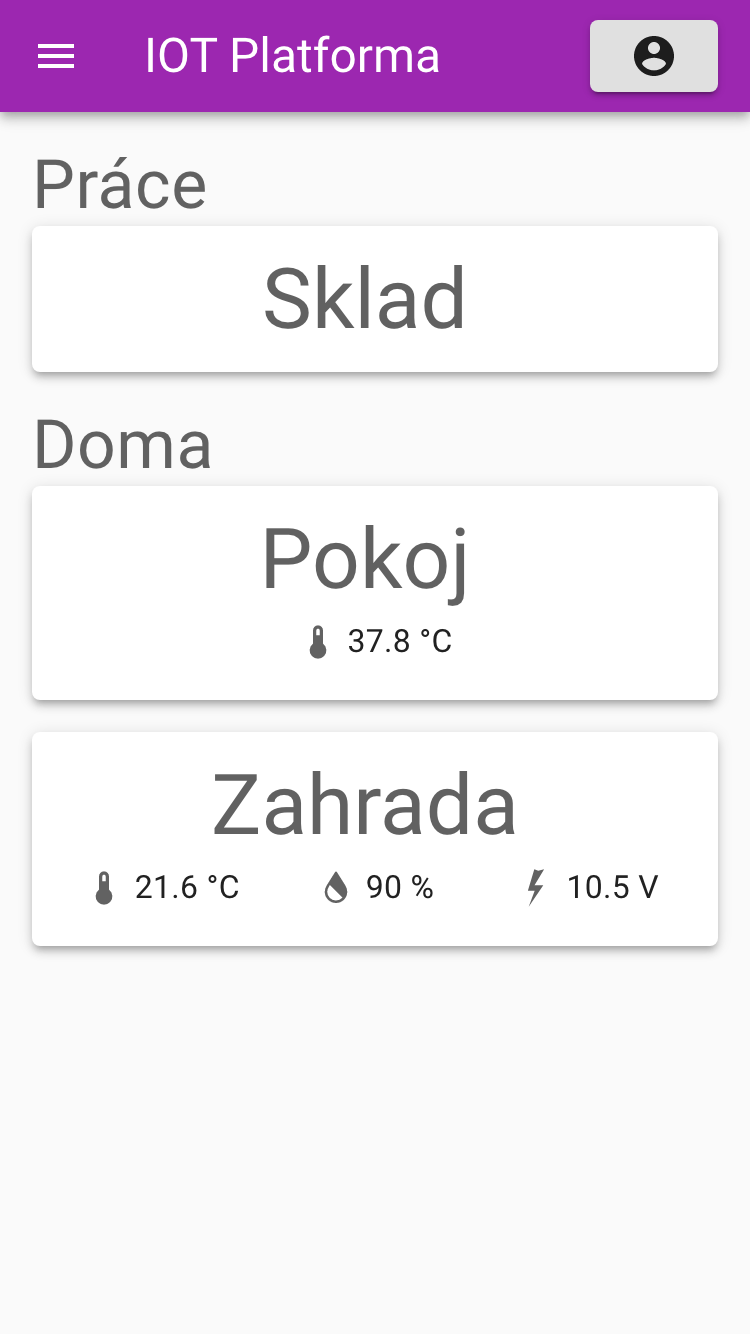
\includegraphics[width=.5\linewidth]{img/screens/buildings.png}
        \caption{Zobrazení místností}
        \label{fig:sub1}
    \end{subfigure}%
    \begin{subfigure}{.5\textwidth}
        \centering
        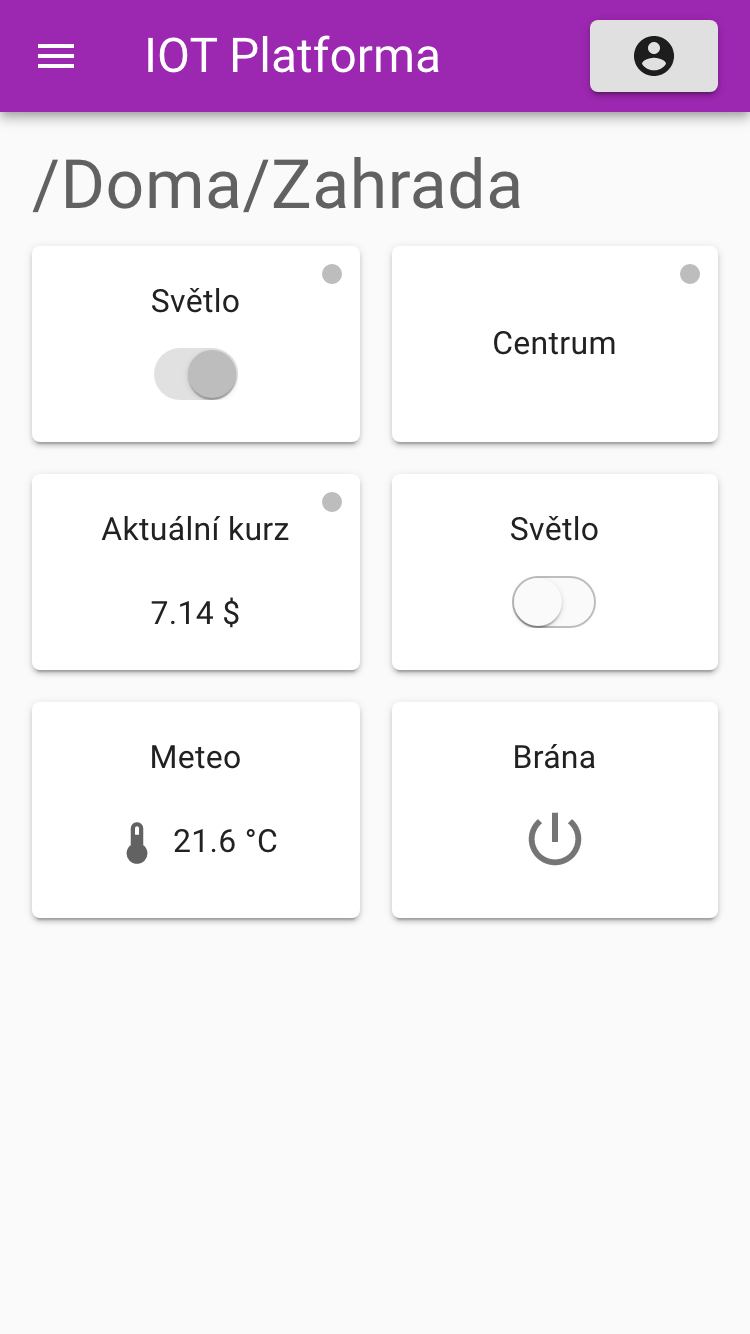
\includegraphics[width=.5\linewidth]{img/screens/room.png}
        \caption{Zobrazení místnosti}
        \label{fig:sub2}
    \end{subfigure}
    \caption{Ukázka rozhraní - výpis místností a jednotlivých věcí v místnosti}
    \label{fig:test}
\end{figure}

Přihlášený uživatel má dále k dispozici menu s možností editace vlastního uživatelskéhoo účtu a odhlášení.

Pokud má uživatel administrátorské oprávnění, tak má navíc k dispozici stránku pro správu uživatelů, ve které je tabulka zobrazující všechny uživatele s možností jejich editace a odstranění.

